\chapter[Multicore designs]{Multicore designs}
\label{cha:multicore}

The purpose of this chapter is to describe in detail the multicore
support that is offered by \ee\ and by \rtd, highlighting the various
features available.




\section[Multicore Design Flow]
{Multicore Design Flow}
\label{sec:multicore-designflow}

The purpose of this section is to shortly describe the design flow
that must be used to develop a multicore system using the tools
provided by Altera and by Evidence Srl. As it can be seen, the design
flow is equivalent to the current Altera design flow, with some
additional points that are needed to create \ee\ compatible hardware
and software.

The first step of a Nios II multicore system is the multicore
hardware. A multicore hardware can be obtained easily using Altera
SOPCBuilder, as described in the document named ``The Multiprocessor
Nios II Systems Tutorial'' \cite{Altera-multicpu-tutorial} that
describes the basics of designing a multicore Nios II system. Please
refer to that document for the basic informations on how to create a
generic Nios II multicore hardware.

Multicore designs compatible with \ee\ can be built starting from the
standard peripherals provided by Altera. For a multicore design to be
compatible with \ee, special care have to be taken when instantiating
particular Altera peripherals and memories. Please refer to the
following sections for the guidelines to be followed when adding the
following hardware features:
\begin{itemize}
\item Interprocessor Interrupt (see Section
  \ref{sec:interprocessor-interrupt});
\item Altera Avalon Mutex (see Section \ref{sec:altera-mutex});
\item Memories (see Section \ref{sec:memories});
\end{itemize}

A step-by-step description on how to create a multicore hardware is
also available inside the ``ERIKA Enterprise Multicore Tutorial for
the Nios II hardware'', available for download at the Evidence web
site.

Once the hardware design has been defined, the designer can develop
the application software using Altera Nios II IDE (based on the Eclipse
Framework).

For each CPU in the system, the designerhave to instantiate an Altera System
Library Project. Please refer to ``The
Multiprocessor Nios II Systems Tutorial'' \cite{Altera-multicpu-tutorial}
for details.

After creating an Altera System Library for each CPU, the designer can
create an \rtd\ Project. The \rtd\ Project contains the application
that will run on {\em all} processors of the system. In a way similar
to the single CPU designs for \ee, the \rtd\ Project contains an OIL
configuration file. The OIL file \cite{OSEKOIL} specifies the
partitioning scheme adopted by a particular application. \rtd\
Projects are described in Section \ref{sec:niosII-basic-notions}.

Next, the designer compiles the application to create a set of
compiled files that are equivalent to the files generated by the
normal Altera Projects makefiles. As a result, the developer can debug
the multicore application as usual using an Altera Multiprocessor
Collection. Please refer to ``The Multiprocessor Nios II Systems
Tutorial'' \cite{Altera-multicpu-tutorial} for details.















\section[Basic notions]{Basic notions for multicore programming}
\label{sec:niosII-basic-notions}

This Section is a simple list of definitions and general terms that
highlight characteristics of the systems that can be designed
using \rtd\ and \ee.

\paragraph{A single SOPCBuilder Block.}
Multicore systems handled by \ee\ are defined inside
a single SOPCBuilder block. This is somehow similar to the approach
followed by ``The Multiprocessor Nios II Systems Tutorial''
\cite{Altera-multicpu-tutorial}.

\paragraph{Partitioning of tasks and data on multicores.}
When developing a multicore system, the user have to think as the
application as a whole. The application will be composed by a set of
tasks, shared resources, that will work cooperatively to reach the
application goals. The approach chosen by \ee\ is a so
called {\em partitioning} approach, that is, each concurrent task is
statically linked at build time to a given CPU. Each CPU includes a
separate copy of the operating system and of the device drivers that
are present on the particular CPU.

Tasks partitioning into CPUs can be done at the end of the application
design: the configuration system is in fact designed in a way to allow
the designer to write partitioning-independent code; then, the
developer can change the CPU partitions without changing the
application source code, giving the possibility to really exploit the
power of Nios II multicores.

The minimal partitioning item in a system is the source file. That is,
the code of tasks allocated to different CPUs are typically put by
designers on different files, to allow an easy partitioning in
different CPU in a later stage of the development.

\paragraph{CPUs are not identical.}
There are various differences between the different CPUs in a
SOPCBuilder Block. First of all, they may come from different versions
of the Nios II core, with possibly different custom
instructions. Moreover, Nios II peripherals are typically connected to
a single CPU\footnote{With the exception of the Altera Avalon Mutex
Peripheral}, and that means that each CPU will have a different set of
interrupts, memories, and software device drivers.

\paragraph{The Master CPU.} 
There is a CPU\footnote{With Nios II 5.0 and 5.1, it was the CPU with
CPUID equal to 0, that wast typically the first CPU in the SOPCBuilder
CPU list.} which plays an important role in the system. That CPU is
usually called {\em \myidx{Master CPU}} and is referred in the source
code as \const{MASTER_CPU}.

In multicore systems supported by \ee, the Master CPU plays an
important role, because it acts as the CPU that have to initialize the
shared data (see Section \ref{sec:memories} and, if configured, the
startup barrier (see Section \ref{sec:startup-barrier}).

The Master CPU is specified in the OIL configuration file as described
in the following example, where \const{cpu0} is specified as the Master CPU:

\index{OIL Example}
\begin{lstlisting}
CPU test_application {
  OS EE {
    ...
    MASTER_CPU = "cpu0";			
    CPU_DATA = NIOSII {
      ID = "cpu0";
      ...
    };
  ...
};
\end{lstlisting}

\paragraph{Altera mutexes.}
The multicore system must include at least an \myidx{Altera Avalon
Mutex peripheral}. That peripheral will be handled internally by \ee\
to guarantee mutual exclusion between different activities residing on
different CPUs (see Section \ref{sec:altera-mutex}). The application
does not use directly the mutex peripheral. If a startup barrier is
configured, a proper initialization value for the mutex have to be
selected (see Section \ref{sec:startup-barrier}).

\paragraph{Multicore Interrupts.}
The multicore system must include a Multicore Interrupt feature. When
developing a multicore application, the designer have only to think at
the existence of concurrent tasks that will be activated and scheduled
on the different CPUs. \ee\ hides the implementation details to the
developer, and the developer does not have to handle the multicore
communication issues. Internally, \ee\ uses a Multicore Interrupt
hardware support, that is used to dispatch various information between
the various CPUs. The instantiation of an Interprocessor Interrupt
peripheral is done connecting together a set of Altera Avalon PIO
components in SOPCBuilder (see Section
\ref{sec:interprocessor-interrupt} on how to instantiate a proper
Multicore Interrupt controller).

\paragraph{Shared Memories.}
A multicore system typically includes some shared memory (that can be
on-chip or off-chip). Shared memories will be used to exchange
informations between the different CPUs. The main idea is that the
designer has the option of defining data structures that are global
and visible to all cores. Moreover, all the CPUs will access the data
structures using an automatic cache disabling technique without
changing the application source code\footnote{Please remember that
Altera Nios II does not have a cache coherency mechanism.}. This kind
of shared data structures will be defined inside the Master
CPU. 

Moreover, the designer can define a shared data structure leaving
\rtd\ the choice if that data structure should be local to a CPU or
global to all the CPUs in the system. The rationale behind this is
that local shared data structures are more efficient than global data
structures, and also the fact that a shared data structure must be
local to a CPU or global depends on the partitioning that the designer
defines for the application. Leaving the choice to \rtd\ allows
designer to write partitioning independent code. See Section
\ref{sec:memories} for details.

\paragraph{\rtd\ project and Altera System Libraries.}
The Nios II IDE project layout for an \ee\ Application slightly differ
from the Altera counterpart. In particular, the user has to
instantiate a Nios II IDE system library for each CPU. \ee\ allows
users to reuse all their preexisting source code developed for the
Altera HAL, adding multiprogramming support to ease the partitioning
job and to fully utilize the multicore power available with Altera
Nios II. Then, the user application is set up inside a \rtd\
Project. An \rtd\ Project is similar to an Altera C/C++ Application
Project, except that an \rtd\ Project includes the application
software for all the CPUs. The partitioning of the application tasks
to processors is specified using a configuration file written
following the OSEK OIL Standard \cite{OSEKOIL}. The result of the
compilation is an ELF file for each CPU, that can be processed in the
same way as the ones produced by normal Altera Nios II Projects. When
compiling an \rtd\ project, Figure \ref{fig:altera-workflow} and
\ref{fig:evidence-workflow} graphically shows the differences between
the various versions: the Altera HAL approach provides a C/C++
application project for each CPU, whereas \ee\ has only one project
(the \rtd\ project) for all the CPUs. Please refer to the \rtd\ manual
on how to create a new \rtd\ Project.

%
\begin{figure}
\includegraphics[%
  width=1\columnwidth]{images/workflow_altera.eps}
\caption{\label{fig:altera-workflow}This Figure displays the Altera
approach to software development with multicore Nios II designs. In
particular, there is one Application for each CPU. each application is
linked to a System Library project, which is linked to the CPU
instantiated in SOPCBuilder.}
\end{figure}

%
\begin{figure}
\includegraphics[%
  width=1\columnwidth]{images/workflow_evidence.eps}
\caption{\label{fig:evidence-workflow}This Figure displays the
Evidence Srl approach to software development with Nios II IDE. In
particular, there is only a single application for every CPU,
contained inside the \rtd\ Project. The \rtd\ project contains the
Application partitioning and the kernel configuration inside the OIL
file. In this sense, the single CPU case showed in Figure
\ref{fig:evidence-single-workflow} is a special case of this
Figure. Then, each CPU has its own System Library, which is linked to
the CPU instantiated in SPCBuilder.}
\end{figure}





\section[Data scopes]{Data scopes in an \ee\ multicore system}
\label{sec:data_scope}

Data allocation in multicore systems based on the Nios II processor
are a little bit different than conventional single processor
architectures. In particular, a C data definition may be classified in
one of the following points.

\paragraph{\myidx{Automatic data}.}

These data are allocated on the current stack by a function call when
the function is called. The scope of these data is the function
itself. Example:

\begin{lstlisting}
void foobar(void)
{
	int this_is_automatic;
	...
}
\end{lstlisting}

% ----------------------------------
\paragraph{\myidx{Static data}.}

Static data is a C global variable that is defined as
\fn{static}. Only the source code inside a file that define the static
variable can refer to the particular symbol.

Example:

\begin{lstlisting}
  static int this_is_static;
\end{lstlisting}

% ----------------------------------
\paragraph{\myidx{Global data}.}

Global data are C global symbols. The scope of these symbols is the
entire source code that is linked inside an ELF file. That is, global
data is {\bf not} shared among different CPUs. Global data is also
called {\em \myidx{Local data}} (to emphasize the fact that they are
allocated to a single CPU only).

\begin{lstlisting}
  int this_is_global;
\end{lstlisting}

% ----------------------------------
\paragraph{\myidx{Heap}.}

Heap data structure are region of memory that are allocated
dynamically using library functions such as \fn{malloc()} and
\fn{free()}.  Typically, each processor has its own private heap
memory pool, that each processor handles independently using a local
copy of the above mentioned Standard C library functions.

Application data structures allocated in the heap typically are local
to each processor and should not be shared among different processors.
\ee\ does not give any explicit support to share a heap variable
(typically a pointer) between tasks allocated to different
processors. To do that, the developer must ensure that:
\begin{itemize}

\item the heap memory resides on a memory zone accessible by the
  different processors that access it;

\item proper cache disabling strategies are used to ensure that each
  processor uses the data consistently;

\item the memory is allocated and freed on the same processor (that
is, the developer cannot allocate a data structure on CPU $a$ and free
it on CPU $b$, because it would have called two different independent
allocators, the allocator on CPU $a$, and the allocator on CPU $b$).


\end{itemize}

% ----------------------------------
\paragraph{\myidx{Multicore global data}.}


Multicore global data are data structures that are visible to {\bf
all} CPUs in the system. This kind of data structure does not exist on
a single processor system. These data structures are typically defined
and initialized inside the \myidx{Master CPU}, and the are accessible
to all the other CPU.

The Multicore Global data must be accessible to all the CPUs, that is,
it must reside on a memory accessible to all the CPUs. As an
alternative, the user can let the memory be shared among the CPUs that
really uses the shared memory, plus the Master CPU (This may help
saving some LE reducing the arbitration logic). Multicore global data
not shared by the Master CPU is not supported in this release of \ee\
(but will probably be supported in future releases).

When a CPU access a multicore global data, the data cache, if present,
is automatically disabled\footnote{Without the need of changing the
source code, using bit-31 cache disabling.}.

% ----------------------------------
\paragraph{\myidx{Stack}.}

The stack memory is used to store function calls, return address, and
parameters. Each task in \ee\ has a stack, that may be shared with
other threads to reduce the overall stack space required by an
application.

Basically, each CPU has stack called "shared"\index{Stack, shared},
that is a fixed size amount that can be specified in the OIL
configuration file. The shared stack has its top at the top of stack
specified for each CPU inside the Altera System Library. That is, the
main() function is always run on the shared stack (that is the same
behavior of normal Altera HAL applications.

Additionally, each task in the system can have a \myidx{private
stack}. A private stack is always needed if the task use blocking
primitives like, for example, WaitEvent. Private stacks are allocated
on the same CPU where the task is allocated.






\section{Memory types and their allocation}
\label{sec:memories}

Altera SOPCBuilder provides the user different kinds of memory types,
ranging from onchip tightly coupled memories, onchip memories, and
external SRAM, SDRAM and Flash memories.

All these different kind of memories can be used to store data and
code. To let the content of a memory being shared among tasks allocated to
different processors, the the memory slave ports must be connected to
all the CPUs that access them.

In general, we will consider a system composed by a set of CPUs that
have some ``private'' memory components (connected to that CPU only),
and a set of ``shared memory'' components (connected to all the CPUs).

In the following, we will consider that the shared memories are
connected to all the available CPUs. Having memories connected to all
the CPUs has the following drawbacks:

\begin{itemize}
\item If a CPU does not need any data structure allocated on a
  particular memory component, the connection logic used to connect
  that CPU to the memory component is wasted. In any case,
  unused arbitration logic can be removed in the final product if
  needed.

\item Having a fully connected memory helps partitioning tasks to
  different processors without changing the hardware. That is
  especially helpful at design phase, where task partitioning is not
  definitive.

\item Fully connected memories, allows a proper handling of the system
  startup. The idea is that the \myidx{Master CPU} have a
  role of ``container'' and ``allocator'' of all the shared data
  structures in the system. All the definitions of the shared data
  structures are done in the Master CPU. Having a single CPU
  responsible for the allocation of the shared data structures
  simplifies the system architecture because the linker takes care of
  allocating shared data structures to separate addresses.

  In this way, \ee\ frees the designer the need to manually allocate
  shared data structures to separate memory zones, that at the end
  forces the developer to manually implement the linker job.
\end{itemize}

Using fully connected memories has the additional advantage of
automatically adapting to partitioning changes, because inserting new
shared data structures (for example because the designer splits a task
in two parts allocated to different processors), or removing existing
multicore shared data structures (because using proper
partitioning data structures that were multicore global may
become local when all the tasks accessing it are allocated on the same
CPU) is handled {\em automatically} by \rtd\ and \ee,
without requiring any kind of manual configuration or, worse, hardware
change.

Please note that whether for simple applications partitioning code and
data structures is a human manageable task, when the application size
grows the complexity of the configuration may be source of human errors
and inefficiencies, especially if the development requires
partitioning changes during system development.

The approach proposed by \rtd\ and \ee\ allows a simple way to
manage the partitioning problem, helping the designer concentrating on
the application architecture instead of concentrating on the
communication support of the application. After the application is
developed, the partitioning will also influence the kind of
communication pattern used to access the data structures. All that is
done only at the software level, without modifying the hardware.

Memory allocation for the application data structures works as follows:

\begin{itemize}
\item The developer defines its data structure.  See Section
  \ref{sec:multicore-shared-data} on how to define a
  multicore shared data structure; see Section
  \ref{sec:GP-disabling} about a discussion on GP-relative
  addressing for multicore global data.

\item The linker allocates the data structures into memory sections,
  that are then located inside the memory components available in the
  hardware. The available memory sections are typically found in the
  Altera generated linker script in the System Library of each
  CPU\footnote{Note that developers may specify their own custom
  linker script.}.

\item The only requirement that have to be fulfilled in this phase is
  that multicore global data structures must be allocated in
  memories that are connected to the various CPUs that may access the
  data. Since memories offsets in the address space are common to all
  the CPUs, pointers and addresses can be shared freely.

  There is no restriction in the allocation of local variables (except
  the obvious one that variables local to a CPU must be allocated in a
  memory space that is accessible by that CPU). Of course, local
  variables should be allocated in preference to private memories.

  Note: when the \rtd\ Code Generator generates the \ee\ configuration
  code for a multicore system, some multicore shared data
  structures are generated. By default, these data structures are
  allocated inside the \const{.rodata}, \const{.sdata} and
  \const{.data} section of the Master CPU. As an alternative, a
  different memory region for the code generated by \rtd\ can be
  selected by specyfying the \const{MP\_SHARED\_RAM} and
  \const{MP\_SHARED\_ROM} attributes in the OIL file. The following
  example shows how the code generated by \rtd\ can be allocated on
  two memories \const{.myram} and \const{.myrom}:

\index{OIL Example}
\begin{lstlisting}
CPU test_application {
  OS EE {
    MP_SHARED_RAM = "__attribute__ ((section (".myram")))";
    MP_SHARED_ROM = "__attribute__ ((section (".myrom")))";
    ...
  };
  ...
};
\end{lstlisting}


\item Since the allocation of multicore data is done
  automatically by the linker, the design of a multicore system
  should take care of the fact that more than one CPU can access the
  same memory component at the same time for data that may be
  uncorrelated. That is, the bandwidth of the memory component is
  shared between different tasks that may access multicore global
  data structures that are not correlated, eventually creating
  bottlenecks.  Such situations can be prevented by appropriately
  fragmenting memory components if possible, allowing decoupled
  parallel access to the different banks (for example, instead of
  having a big onchip memory of 64Kb, having 2 32k memories with an
  appropriate partition of the data structures).
\end{itemize}





\section{Handling data consistency using mutual exclusion}
\label{sec:altera-mutex}

Whenever a data structure can be accessed concurrently by different
tasks, a mutual exclusion mechanism must be used to ensure that the
shared data structure is accessed without consistency problems.

\ee\ provides a mutual exclusion mechanism between concurrent tasks
through the abstraction of \myidx{Resource}. Resources are similar to
binary semaphores, and can be locked using the \reffun{GetResource}
primitive and released using the \reffun{ReleaseResource} primitive.

A Resource is modeled using an \ee\ Resource object, that can be
thought as a binary semaphore plus a rule that says that when a task
$\alpha$ allocated on a CPU tries to lock a resource locked by another
task $\beta$ on another CPU, then $\alpha$ actively spins waiting for
$\beta$ to release the lock. This protocol is also called
Multiprocessor Stack Resource Policy (MSRP)
%
%
% Nota: aggiungere un riferimento quando il capitolo di peppe sara' pronto
%
%\ref{XXX-capitoloMSRP}).
%
%

These primitives can be used by tasks independently from the CPU where
the tasks are allocated to. The \rtd\ Code Generator, and the
implementation of the primitives done on \ee, guarantees that
GetResource and ReleaseResource can be transparently remapped to
multicore platform, hiding the complexity of the multicore platform.

Basically, the \rtd\ Code Generator handles in a different way
Resources that are used only by task allocated to the same CPU ({\em
local} resources \index{local resources}) and Resources that are used
by tasks allocated to different CPUs ({\em global} resources
\index{global resources}). 

Locking a local resource only provoke a modification in the scheduling
parameters on the local CPU, whereas locking global resources involve
a coordination between tasks allocated to different CPUs that is
solved by the \ee\ using an \myidx{Altera Avalon Mutex} peripheral
internally.

The kind of lock implementation used for a particular resource only
depends on the partitioning defined in the OIL file.  Please note that
developers does not have to modify their code after a system
repartitioning that changes a resource from local to global or vice versa.

The options that influence Resources and their allocation in the OIL
configuration file are described in the following example:

\index{OIL Example}
\begin{lstlisting}
CPU test_application {
  OS EE {
    NIOS2_MUTEX_BASE = "MUTEX_BASE";
    ...
  };

  TASK thread0 {
    CPU_ID = "cpu0";
    RESOURCE = myresource;
    ...
  };

  RESOURCE myresource {
    RESOURCEPROPERTY = STANDARD { APP_SRC = "resourcedata.c"; };
  };

  ...
};
\end{lstlisting}

Basically, the developer have to specify inside the property
\const{NIOS2_MUTEX_BASE}\index{NIOS2\_MUTEX\_BASE} the base address that
is generated by the system library inside the \file{system.h}
file. The name of the base address is typically the name used in
SOPCBuilder (uppercase), plus the suffix \const{_BASE}. For example,
for a mutex device called \const{mutex}, then the name of the base
address to be used is \const{MUTEX_BASE}. Then each thread have to
declare the resources it use. Finally, the Resource have to be
declared, eventually specifying additional source files. When
generating the configuration code, if the Resource will be local,
these source files will be linked to the CPU where the tasks that use
it are allocated; otherwise, the source files will be linked together
with the \myidx{Master CPU}.

Please note that (starting from Nios II 6.0, the \ee\ implementation
does no more use the HAL mutex driver, but it uses its own mutex
driver.





\section{\myidx{Startup barrier}}
\label{sec:startup-barrier}

Each processor in a multicore environment is characterized by a
different set of peripherals, a different size of code and data
structures. As a drawback, each CPU will have a different startup code
implying that each CPU will have a different boot time (let's consider
the boot time the time from the CPU reset to the execution of the
first assembler instruction of the \fn{main()} function).

Since the different CPUs will execute a set of interacting code, it is
important that all the CPU execution will be synchronized before they
start the application, giving in that way the time to all the CPUs to
startup their peripherals, and to properly initialize their global
data structures. We call that initial synchronization a "startup
barrier".

\ee\ provides an (optional) startup barrier service. When configured
and correctly used, the CPUs will run the boot code, and will stop at
a synchronization point inside the \fn{StartOS()}\index{StartOS}
primitive until all the CPUs have passed it.

The implementation of the startup barrier uses the services of the
\myidx{Altera Avalon Mutex} peripheral. In
particular, to implement the startup barrier we used the {\em Initial
Owner} feature as shown in Figure \ref{fig:sopcbuilder-mutex}.

%
\begin{figure}
  \begin{center}
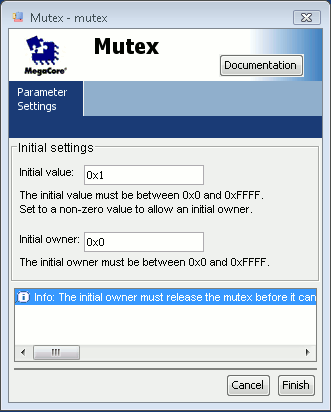
\includegraphics[%
  width=8cm, bb=0 0 331 412]{images/SOPCBuilder_Mutex.png}
  \end{center}
\caption{\label{fig:sopcbuilder-mutex}This Figure displays the {\em
Initial Value} and the {\em Initial Owner} setup for the Altera Avalon
Mutex peripheral. The setting must be different from 0 only when using
the startup barrier feature. }
\end{figure}

The settings to be used when configuring the startup barrier are the
following: 

\begin{itemize}
\item The Altera Avalon Mutex initialization values are set according
  to Figure \ref{fig:sopcbuilder-mutex}. Please note that if you are
  using Nios II version 6.0, the value $0$ is set in any case and it
  has \bf{no relationship} with the CPUID register values assigned by
  SOPCBuilder\footnote{If you are using Nios II versions 5.0 and 5.1,
  $0$ is the CPUID register value for the first CPU.}.

\item The first cpu that is listed in the OIL file is the first CPU
  that is listed in SOPCBuilder (in this way, \rtd\ will assign
  that CPU the index $0$.

\item The \myidx{Master CPU} setting in the OIL file is set
  to the first CPU, and the \const{STARTUPSYNC} value is set to
  \const{TRUE} as shown below: 
\index{OIL Example}
\begin{lstlisting}
CPU test_application {
  OS EE {
    MASTER_CPU = "cpu0";			
    CPU_DATA = NIOSII {
      ID = "cpu0";
      ...
    };
    
    CPU_DATA = NIOSII {
      ID = "cpu1";
      ...
    };
    
    STARTUPSYNC = TRUE;
    ...
};
...
\end{lstlisting}

\end{itemize}

If you want not to configure the startup barrier, you have to set all
the initialization values of the Altera Avalon mutex to 0, and the
\const{STARTUPSYNC} value to \const{FALSE}\footnote{By default, the
binary distributions of \ee\ do not allow the possibility to remove
the startup barrier.}.

\begin{warning}
If you are using Nios II 5.0 or 5.1, please read the following
paragraphs.  Please note that unfortunately Altera does not guarantee
an assignment pattern to the CPUID (\const{ctrl5}) values. The CPUID
values are assigned in an automatic way by SOPCBuilder, and the user
does not have control over it. For that reason, the value that is set
as initialization value for the Altera Avalon Mutex may be not what
the user would like to. In our experiments, we found that an
initialization value of 0 typically corresponded to the first CPU in
SOPCBuilder, but unfortunately there is nothing that really specifies
the assignment strategy of CPUIDs done by SOPCBuilder.

To check the correctness of the initialization value of the startup
barrier, a designer can do the following procedure:
\begin{itemize}
\item The designer creates the multicore system, including the
  Altera Avalon Mutex.

\item Then, the user have to check the value of the CPUID register for
  the first CPU. To do that, please open the PTF file containing the
  system description. Inside the \const{MODULE} section of the various
  CPUs, search for the \const{WIZARD_SCRIPT_ARGUMENTS} section. Look
  at the value for the attribute \const{cpuid_value}: that is the
  CPUID value for the considered CPU.

\item The value found in the previous step for the \myidx{Master CPU}
  must be equal to the {\em Initial Owner} that is set in the Altera
  Avalon Mutex dialog box (see Figure \ref{fig:sopcbuilder-mutex}).
\end{itemize}
\end{warning}

\begin{warning}
Typical behavior that shows up when the mutex initialization is not
done in the proper ways is that the either system (all the CPUs)
simply blocks at the startup barrier, or simply the barrier is not
considered at all. The latter case is subtle because some of the
processors could start to use the shared data structures when the CPU
responsible for their initialization has not initialized them yet. In
this case the early arriving processor could have read uninitialized
values, and the values written could be overwritten by the
initialization values.
\end{warning}

\begin{warning}
Please note that the initialization value of the Altera Avalon Mutex
done with the startup barrier is only valid when the system boots up
the first time. When debugging a multicore systems with a startup
barrier\index{Startup Barrier}, the user have to reboot {\em all} the
CPUs when starting a multicore debug system. Simply stopping the
debugger and starting another debug session in the Nios II IDE is not
sufficient, because the Altera Mutex is not reset.
\end{warning}

%% The startup barrier is basically needed for the following reason:

%% \begin{itemize}
%% \item there exist a set of CPUs using concurrently certain
%%   multicore global data structures

%% \item the multicore global data structures are typically defined
%%   and initialized by the first CPU, and then shared with the other
%%   CPUs as external data

%% \item the system startup routine of the multicore system must
%%   initialize the multicore global data structures, and the
%%   initialization time may require a time that depends on the number of
%%   peripherals attached to the CPUs, to the size of the data structures
%%   that are defined by the CPU (in general they can be global or
%%   multicore global)

%% \item for these reasons, when the system starts, all the CPUs have a
%%   different initialization time, and only when all the CPUs have
%%   finished their initialization they can start using the
%%   multicore system.

%% \end{itemize}







\section{\myidx{Interprocessor Interrupt}}
\label{sec:interprocessor-interrupt}

Multicore Nios II systems using \ee\ must include an Interprocessor
Interrupt Controller in order for a CPU to notify events to other
CPUs. For that reason, Evidence SRL supports interprocessor interrupt
controllers for up to 32 processors, made using the standard Altera
Avalon PIO SOPCBuilder Component.

Once included into the design, the Interprocessor interrupt feature
will be used internally by \ee. The developer does not have to care
anymore about it.

The interprocessor interrupt is made by two main parts, the {\em
input} part and the {\em output} part. It has to be created following
these guidelines:




\begin{itemize}

\item First of all, the designer have to instantiate the {\em input}
  part of the Interprocessor Interrupt controller, that is basically
  an Altera Avalon PIO component for each CPU in the system. The
  component must be an input PIO, capable to raise an interrupts on
  the rising edge of the input pin. Figures
  \ref{fig:IPIC-input-basic}, \ref{fig:IPIC-input-input}, and
  \ref{fig:IPIC-input-simulation} shows the settings to be used for
  each component. The components have to be connected to each CPU data
  master. The Interrupt priority should be the lowest among the
  priorities of the interrupts connected to a given CPU.

\item Then, the designer have to instantiate the {\em output} part of
  the Interprocessor interrupt controller, that is basically a
  system wide Altera Avalon output PIO component. The component must
  have 1 output bit {\em for each} CPU in the system. Figure
  \ref{fig:IPIC-output} shows a 2 CPU setting for this component. The
  component have to be connected to the data master of {\em all} the
  CPUs.

\item After that, the input part and the output part of the
  Interprocessor Interrupt have to be connected together. The simplest
  way to do that is from the BDF file containing the SOPCBuilder
  Component. After generating the SOPCBuilder Component, please
  connect each output pin of the output PIO to a correspondent 1-pin
  input PIO. Figure \ref{fig:IPIC-out-2cpu} and \ref{fig:IPIC-in-2cpu}
  show a simple way to connect them using Altera Quartus II named
  pins. The pins have to be connected {\em in the same order specified
  in the CPUID register} of each CPU. That is, the CPU with
  \const{CPUID} 0 have to be connected to the pin 0 of the output PIO,
  and so on.

\item Next, in the OIL configuration file, the CPU have to be listed
  (again) in the order of the CPUID register, that is the same order
  they are connected to the interprocessor Interrupt output pins,
  starting from 0. An example for the 2 CPU snapshots showed in
  Figure \ref{fig:IPIC-out-2cpu} and \ref{fig:IPIC-in-2cpu} is
  included below. The \const{IPIC_GLOBAL_NAME} contains the uppercase
  name of the IPIC output part, as listed in the \file{system.h} file
  generated by the Altera System Libraries.  The
  \const{IPIC_LOCAL_NAME} contains the uppercase name of the IPIC
  input part, as listed in the \file{system.h} file generated by the
  Altera System Libraries for each CPU.

\index{OIL Example}
\begin{lstlisting}
CPU test_application {
  OS EE {
    ...
    MASTER_CPU = "cpu0";			
    IPIC_GLOBAL_NAME = "IPIC_OUTPUT";
    CPU_DATA = NIOSII {
      ID = "cpu0";
      IPIC_LOCAL_NAME = "IPIC_INPUT_CPU0";
      ...
    };
    CPU_DATA = NIOSII {
      ID = "cpu1";
      IPIC_LOCAL_NAME = "IPIC_INPUT_CPU1";
      ...
    };
    ...
  };
  ...
};
\end{lstlisting}



\item Finally, \ee\ will take care of the interprocessor interrupt
  code. The only thing the user have to specify is the CPU where each
  task have to be executed; the \rtd\ code generator will configure
  \ee\ to automatically use interprocessor interrupts when needed.
\end{itemize}

\begin{figure}
  \begin{center}
    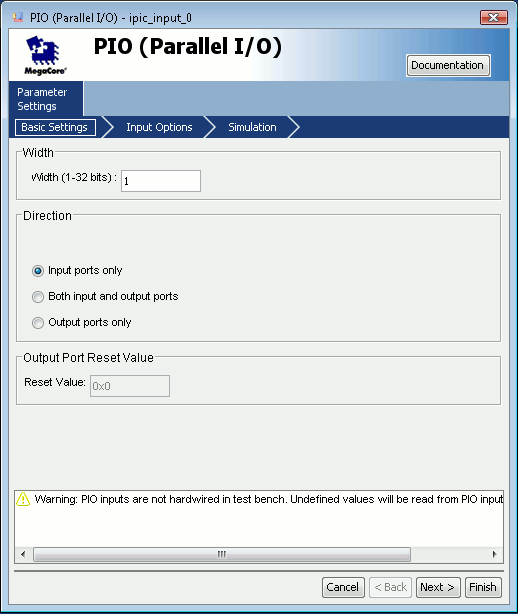
\includegraphics[width=5cm, bb=0 0 518 614]{images/IPIC_PIO_in_dialogbox_basic.png}
  \end{center}
  \caption{Input part of the Interprocessor 
    Interrupt. The Figure shows the Avalon PIO basic settings.}
  \label{fig:IPIC-input-basic}
\end{figure}

\begin{figure}
  \begin{center}
    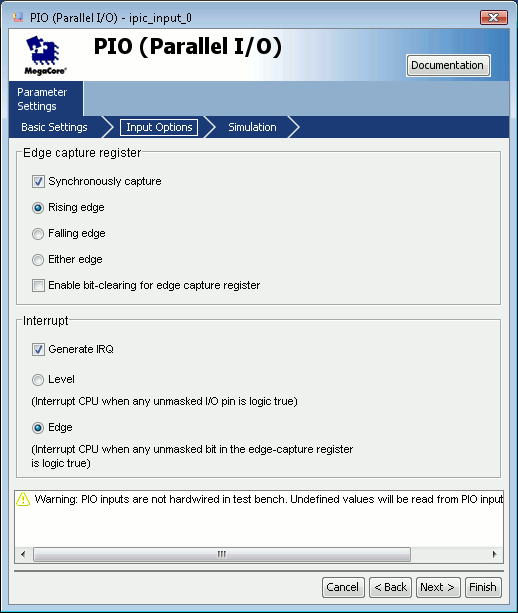
\includegraphics[width=5cm, bb=0 0 518 613]{images/IPIC_PIO_in_dialogbox_input.png}
    %\pgfimage[width=7cm]{images/IPIC_PIO_in_dialogbox_input.png}
  \end{center}
  \caption{Input part of the Interprocessor Interrupt. 
    The Figure shows the Avalon PIO input settings.}
  \label{fig:IPIC-input-input}
\end{figure}

\begin{figure}
  \begin{center}
    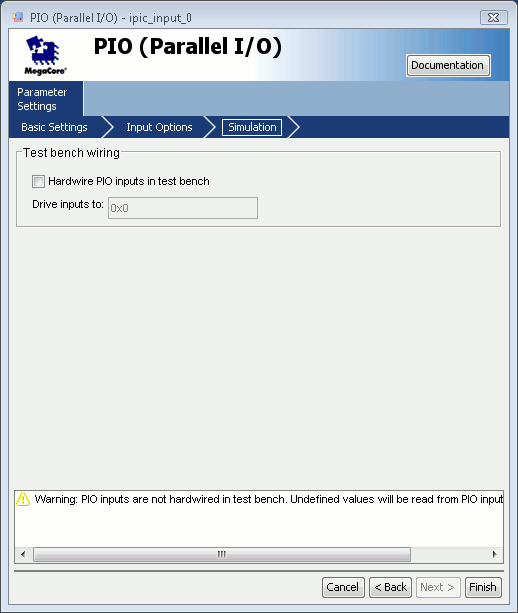
\includegraphics[width=5cm, bb=0 0 518 613]{images/IPIC_PIO_in_dialogbox_simulation.png}
    %\pgfimage{images/IPIC_PIO_in_dialogbox_simulation.png}
  \end{center}
  \caption{Input part of the Interprocessor Interrupt. 
    The Figure shows the Avalon PIO simulation settings.}
  \label{fig:IPIC-input-simulation}
\end{figure}

\begin{figure}
  \begin{center}
    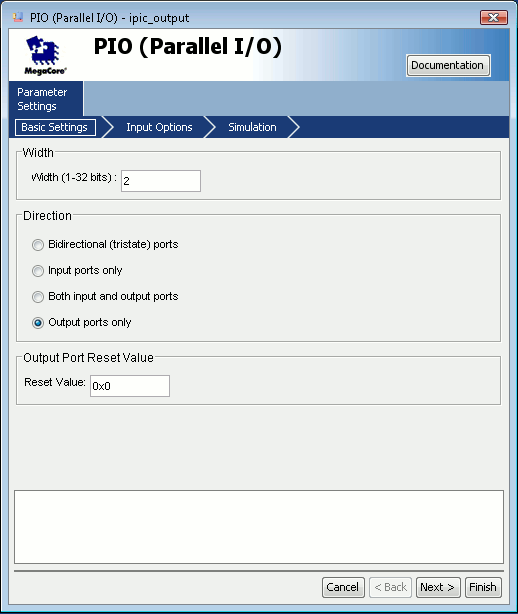
\includegraphics[width=5cm, bb=0 0 518 614]{images/IPIC_PIO_out_dialogbox.png}
    %\pgfimage[width=7cm]{images/IPIC_PIO_out_dialogbox.png}
  \end{center}
  \caption{Output part of the Interprocessor Interrupt. 
    The Figure shows the Avalon PIO output settings.}
  \label{fig:IPIC-output}
\end{figure}

\begin{figure}
  \begin{center}
    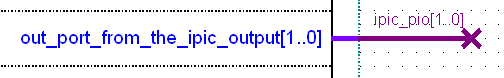
\includegraphics[width=7cm, bb=0 0 504 78]{images/IPIC_PIO_out_2cpu.png}
    %\pgfimage[width=7cm]{images/IPIC_PIO_out_2cpu.png}
  \end{center}
  \caption{Output part of the connection from
    the output PIO of the SOPCBuilder Component to the input PIO in each
    CPU.}
  \label{fig:IPIC-out-2cpu} 
\end{figure}

\begin{figure}
  \begin{center}
    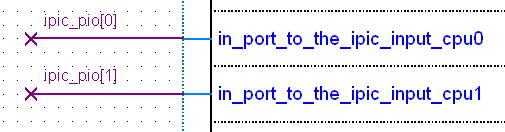
\includegraphics[width=7cm, bb=0 0 505 132]{images/IPIC_PIO_in_2cpu.png}
    %\pgfimage[width=7cm]{images/IPIC_PIO_in_2cpu.png}
  \end{center}
  \caption{Input part of the connection from
    the output PIO of the SOPCBuilder Component to the input PIO in each
    CPU.}
  \label{fig:IPIC-in-2cpu} 
\end{figure}







\section{Data caches and multicore data sharing}
\label{sec:multicore-shared-data}

One of the main problems when dealing with shared memories with multicores is the consistency of shared data structures, that have to be ensured in every condition.

The problem of data consistency for the Nios II
architectures melts down to two topics: one is the mutual exclusion
between data accesses, that is obtained hiding the usage of the Altera
Avalon Mutex peripherals inside the RTOS \fn{GetResource()} and
\fn{ReleaseResource()} primitives (see Section
\ref{sec:altera-mutex}), and the other one is related to the usage of
data caches with multicore shared data.

This section describes the usage of data cache and of data cache
disabling to implement multicore data sharing. Basically, all the
accesses to multicore global data structures in Nios II
architectures must be done using cache disabling techniques, because
the Nios II architecture does not support (yet) cache coherency protocols.

Cache disabling in the Nios II can be obtained using the following methods:
\begin{enumerate}
\item Using IORD/IOWR to explicitly say that a particular access
  must be done using cache disabling;

\item Using tightly coupled memories;

\item Using explicit data cache flushes;

\item Using bit-31 cache disabling;
\end{enumerate}
In most of these cases, (except tightly coupled memories) implementing
a cache disabling mechanism implies an explicit modification of the
source code.

Instead of requiring an explicit code modification at each data
access, \ee\ provides a method for obtaining cache disabling changing
{\em only} the definition of a data structure. That feature is
obtained using the bit-31 cache disabling feature of Nios II, and
allows the implicit use of bit-31 cache disabling to all the accesses
of selected data structures.

The rationale behind using cache disable when dealing with
multicore global data is that the designer must write the
application code in a way {\em independent} from the fact that a
particular data structure is shared or not between tasks allocated to
different processors: that fact indeed depends on the partitioning
specified inside the OIL file. A change in the partitioning may
influence the fact that a data structure is global or not, and the
designer must be as much as possible freed from modifying the code
upon a repartitioning of an application.

Another reason to use implicit cache disabling techniques is the
support for moving legacy single processor code to a multicore system
without changing the source code implementing the application
algorithms, but only changing the data definitions. Again, the idea is
that the source code must be as much as possible independent from the
partitioning scheme chosen by the developer.

As the final thing, since cache disabling reduces the performance of
the system because it basically skips the usage of the CPU data cache
(if present), cache disabling techniques must be used only for
selected data structures, limiting as much as possible the performance
penalty related to cache disabling.


\subsection{How to define cache-disabled multicore global data structures}

\ee\ currently offers two techniques to implement cache disabling:

\paragraph{Cache disabling for all the accesses to a multicore global
  data structure.}

This technique can be used whenever the developer wants to disable the
cache to all the accesses to a particular data structure. In
particular, the user has to {\bf define} the multicore global data
structure using the \const{EE_SHARED_DATA}\index{EE\_SHARED\_DATA}
macro. The following example shows how to use the
\const{EE_SHARED_DATA}macro to define a global structure named
\vr{mystruct}

\begin{lstlisting}
struct mystruct {
  ...
};

volatile struct mystruct EE_SHARED_DATA(foo);    
\end{lstlisting}

In this example, the \vr{foo} variable is defined as {\em shared}, and
all the accesses done to that variable will use the bit-31 cache
disabling technique.

\begin{warning}
All the multicore global data structures must be defined in files
that are compiled by the \const{MASTER_CPU}\index{MASTER\_CPU} specified in the OIL File.

A typical way of doing that is to put all the multicore global
data structures inside a file that is specified in the
\const{MASTER_CPU} CPU section, as in the following example:

\index{OIL Example}
\begin{lstlisting}
CPU test_application {
  OS EE {
    ...
    MASTER_CPU = "cpu0";			
    CPU_DATA = NIOSII {
      ID = "cpu0";
      APP_SRC = "shareddata.c";
      ...
    };
    ...
  };
};
\end{lstlisting}
\end{warning}



\paragraph{Cache disabling for all the access to shared data structures.}

This technique uses cache disabling selectively only on the data
structures that are shared between different CPUs. The idea is that a
multicore application is composed by a set of tasks that uses
shared resources. 

Shared resources are defined inside the OIL file, and for each task it
is specified which resource the task is using (see the OIL example in
Section \ref{sec:altera-mutex}).  Depending on the partitioning of
tasks to CPUs chosen by the designer, the resources can be either {\em
local} (that is, all the tasks using the resources are allocated to
the same CPU, and the data structure can be global to that CPU only),
or {\em global} (that is, the tasks using the resource are allocated
to different CPUs). Only the latter case really needs a cache
disabling mechanism\footnote{Using cache disabling with the
\const{EE_SHARED_DATA} technique is correct but not efficient, because
cache disabling may is used also when a resource become local due to a
repartitioning and thus there would have been to need to use cache
disabling.}

In this case, the \const{EE_SHARED_RES}\index{EE\_SHARED\_RES} macro
must be used.  \const{EE_SHARED_RES} takes an additional parameter,
that is the OIL resource that must be considered for deciding if cache
must be disabled or not. The following examples shows a typical usage
of the macro:

\begin{lstlisting}
volatile struct mystruct EE_SHARED_RES(myresource, foo);
\end{lstlisting}

In this case, the foo data structure will be shared using bit-31 cache
disabling {\em only} when \vr{myresource} is a global resource.

\begin{warning}
Special care must be taken in this case, because the definition of all
the data structures for resource \vr{myresource} must be put in a
separate file. The filename is then listed in the \const{RESOURCE}
section of the \vr{myresource} resource in the OIL file (see the
example below).  If the resource is local, the file will be compiled
together with the CPU where the tasks using it are allocated; if the
resource is global, the file will be compiled together with the
\const{MASTER_CPU}.

\index{OIL Example}
\begin{lstlisting}

CPU test_application {
  ...
  RESOURCE mutex {
    RESOURCEPROPERTY = STANDARD { APP_SRC = "resourcedata.c"; };
  };
};
\end{lstlisting}
\end{warning}







\subsection{How to define a data structure that is global to a 
single processor}

To define a data structure that is global to a single CPU, the
developer must define a traditional C global variable, making sure
that the file that defines the variable is compiled inside the right
CPU. To obtain that, the developer have to list the file containing
the global variable either in the CPU section of the OIL file (look at
\file{mydata1.c}) or in a task allocated to the particular CPU (look
at \file{mydata2.c}), as in the following example:

\index{OIL Example}
\begin{lstlisting}
CPU test_application {
  OS EE {
    ...
    CPU_DATA = NIOSII {
      ID = "mycpu";
      APP_SRC = "mydata1.c";
    };
    ...
    TASK mytask {
      CPU_ID = "mycpu";
      APP_SRC = "mydata2.c";
    };
  };
};    
\end{lstlisting}

 \begin{warning}
The scope of the global definition is the CPU where the data
 structure is compiled. Other CPUs will not have access to that data
 structure symbol, meaning that other CPUs can define symbols with the
 {\em same} name.
\end{warning}


\subsection{How to allocate a data structure inside a particular 
data memory}

In general, to allocate a data structure to a particular memory
region, the user must explicitly use the section attribute of the gcc
compiler, as in the example below. Please note that the memory region
must be visible to the CPU defining it.

\begin{lstlisting}
extern int foobar (void) 
       __attribute__ ((section (".myonchipmemory")));
\end{lstlisting}

\begin{warning}
  If the memory region is not private to a particular CPU, but is
  shared among different CPUs, then the memory region should also be
  visible to the \const{MASTER_CPU}, and the variable that have to be
  allocated on that memory region should be defined in a file that is
  compiled by the \const{MASTER_CPU}.
\end{warning}





\subsection{Disabling GP addressing for global resource access}
\label{sec:GP-disabling}
This section describes a common linking problem when developing
multicore application with shared data, and describes workaround
for it.

The Nios II architecture and the implementation done with the gcc
compiler allows two types of addressing for the data structures: one
is the global addressing, where the compiler generates code to compute
an absolute address that is then used to access the data; the other
method is to maintain a register value containing an absolute address
of a memory region, and then use an offset to that location to access
the memory. Whereas the latter method is more efficient than the
former, it has the limitation that it can access only data structures
that lies in a range +/- 32Kbytes from the address used in the
register.

The gcc compiler uses the second method to access the small data
sections (typically, small data elements like integers, chars, small
structures, ...). In particular, it reserves the \vr{gp} register for this
use.

When using small multicore global data structures, the compiler
continues to generate gp-relative code, but that gp-relative code
cannot be used because bit-31 cache disabling generates an address
that is far beyond the 32Kb offset possible with relative
addressing\footnote{That because the bit 31 of the address is 1.}.

The result is that the compiler generates gp-relative code that at the
end cannot be linked. A typical linker error in this case is the
following:

\begin{lstlisting}
  filename:line: Unable to reach this_is_shared (at 0x82012120) 
  from the global pointer (at 0x0201a064) because the offset 
  (2147451068) is out of the allowed range, -32678 to 32767.
\end{lstlisting}

To avoid this linker error the developer has to tell the compiler to
disable the GP-relative code generation for that data structure. There
are two possible ways that can be used, depending on the final memory
where the data structure can be allocated:

\begin{itemize}
\item if the data structure is allocated in the default memory
  specified in the Altera system library, the developer can use the
  following declaration

  \begin{lstlisting}
extern volatile int this_is_shared EE_DISABLE_GP_ADDRESSING;
  \end{lstlisting}
  (this method works in all the cases).


\item As an alternative to the previous method, if the data structure is
  allocated in a particular memory component, the developer can
  explicitly specify the target memory in the DECLARATION using the
  gcc section attribute command. An example of a typical declaration
  is the following:

  \begin{lstlisting}
extern volatile int goofy 
       __attribute__ ((section (".mymemory")));
  \end{lstlisting}
  Please note that {\bf all} the declaration of the data structure
  must have the sections specified in this way. In general, the gcc
  compiler consider the attribute specified in the latest declaration.
\end{itemize}








\section{Code sharing}

Sharing code among processor can be useful if the designer has need to
reduce the memory footprint used by some parts of source code.

The source code that can be shared among CPUs must have the following
characteristics:

\begin{itemize}

\item The code must only use multicore global data or automatic
  data.


\item The code must be linked to the \const{MASTER_CPU}. For example,
a way to obtain that is to list the file containing the shared code
inside the Master CPU in the OIL file, as in the following example:

\index{OIL Example}
\begin{lstlisting}
CPU test_application {
  OS EE {
    ...
    MASTER_CPU = "cpu0";			
    CPU_DATA = NIOSII {
      ID = "cpu0";
      APP_SRC = "mysharedcode.c";
      ...
    };
  ...
};
\end{lstlisting}



\item The code must reside in a memory that is accessible from the
  other CPUs that needs access to it.

\end{itemize}

\begin{warning}
Please note that a shared code accessing global data (that is, global
symbols visible from the code on the \const{MASTER_CPU} only) may not
work if executed on other processors. NO ERRORS are raised by the
compiler in these situations, so it is up to the developer to check
that everything is generated correctly.
\end{warning}

To share a C function, the user has to use the \const{EE_SHARED_CODE}
macro when defining the function. Here is an example:

\begin{lstlisting}
void EE_SHARED_CODE(foobar)(void) 
{ 
   ...  
}
\end{lstlisting}






\section{On-chip memories, .hex files and multicore systems}
\label{sec:hex-problem}

Onchip memories are special memories that resides inside the
FPGA. Initialization of these memories is done at FPGA reset time when
the FPGA data stream is loaded initializing the hardware
configuration.  When an application is compiled, the initialization
values for onchip memories are created inside \file{.hex} files, and
when the hardware project is assembled the initialization values
written inside the \file{.hex} files are assembled inside the
\file{.sof}. In this way, onchip memories are already initialized upon
FPGA reset.

The initialization of the onchip memories are stored in \file{.hex}
files that have the name of the memory components. The \file{.hex}
files are typically created by the Altera Nios II System
library/Application makefiles. The \file{.hex} files are copied inside
the \file{.sof} file at the assembly phase in Quartus
II. Unfortunately, the Altera Makefile scripts put the \file{.hex}
files inside the hardware project directory (that is, the directory
that also contains the SOPCBuilder block files).

In the case of a multicore system, onchip memories will be often
used to implement data exchange between processors. That means that
more than one CPU will have the right of accessing a particular
onchip memory, and also means that the compilation scripts for all the
CPUs will produce their \file{.hex} files with the initialization of these
memories. In general, the hex files will be the one produced by the
latest compilation of the CPU that can access them.

At the end of the compilation process the \ee\ scripts takes care of
handling the \file{.hex} generation in the following way:

\begin{description}

\item[Onchip memories accessible from one CPU only.] In this
  case, the \file{.hex} file is generated when the CPU ELF file is
  compiled as part of the compilation process. The \file{.hex} file
  contains all the data structures (and their initialization) that the
  user put on that memory using the gcc section attribute. As an
  example, to allocate a data structure inside an onchip memory the
  user has to write:

  \begin{lstlisting}
int foo __attribute__ ((section (".myonchipmemory")));
  \end{lstlisting}
  Please note that if in the Altera System Library Configuration for
  the particular CPU the onchip memory has been defined as the
  privileged memory for data and code, also the corresponding sections
  (.text for code, .data, .sdata, ... for the data) will be inserted
  inside the particular onchip memory.



\item[Onchip memories accessible by different CPUs
  (Master CPU included).]~ 

  In this case, the final \file{.hex} file will be produced when
  compiling the \const{MASTER_CPU}\index{Master CPU}. This is the
  common case where the onchip memories are used for data exchange
  between CPUs: the shared data structures are defined in the Master
  CPU and used by all the other CPUs (other CPUs will have the data
  structure only declared, not defined).  The Master CPU will also
  have the burden of initializing the onchip memory.


\item[Onchip memories accessible by different CPUs
  (Master CPU not included).]~

  This case is currently not handled, and will be probably supported
  in future releases of \ee. The current behavior is that the
  \file{.hex} that is finally produced is the one produced by the
  latest CPU that has been compiled and that can access the
  memory. The current behavior is that the latest CPU is typically the
  latest one in the OIL file (this behavior will not be guaranteed in
  future releases).

  In summary:
  \begin{itemize}
  \item When possible, avoid this case.
  \item If you really need to use it (for example in cases where there
    is no space on the FPGA for the arbitration logic for the Master CPU, or
    when using tightly coupled memories between CPUs different from
    the \const{MASTER_CPU}), try to write the code in a way that it
    will not depend on the initialization values of the data stored in
    that onchip memories.
  \end{itemize}
\end{description}










\section{Designing multicore software}

After having described in the previous sections the basic pieces
composing a multicore application, we are now able to highlight the
architecture of a typical \ee\ multicore application:

\begin{itemize}
\item The platform is defined by a multicore Nios II system composed
  by a set of CPUs. Each CPU has a set of peripheral connected to it,
  plus an Altera Avalon Mutex and an Interprocessor Interrupt
  component.


\item The partitioning scheme used on a given configuration is
  specified inside an OIL configuration file. A a graphical
  configuration plugin for the Nios II IDE will be available in the
  next version.


\item Tasks should be written each one on a different file. Putting
  more than one task on the same file is permitted, although it limits
  the possibilities to partition the two tasks on different CPUs (the
  minimal entity that can be partitioned from one CPU to the others is
  a file). Activating tasks on other CPUs is possible and it is
  handled transparently by the kernel primitives using multicore IRQs.


\item Some data structures will be typically local to a CPU, other
  data structures will be global to all the CPU that exists in the
  system.  Sharing symbols with cache disabling among the various CPUs
  is automatically handled by \ee.


\item Shared data between tasks must be handled using the primitives
  \reffun{GetResource} and \reffun{ReleaseResource} primitives
  independently of the CPU where tasks are allocated. The usage of the
  Altera Avalon Mutex is hided by \ee.


\item Task Activations, Task Event Setting, and Alarm notifications
  that involves them are handled by \ee\ in a way independent from
  which CPU a particular task is allocated to.


\item Counters, Alarms, Application modes, and Hooks are local to a
  given CPU and are not shared between different CPUs.


\item A typical multicore application will consider the fact that a
  set of tasks related to peripheral/interrupt handling should be
  allocated to the CPUs where these peripherals are connected to.
  Eventually these tasks will have to call the Altera HAL peripheral
  primitives. Further processing, and peripheral independent tasks
  will be allocated and partitioned among the various available CPUs.


\item Resources will be dedicated to the exchange of informations
  between the various tasks. Resources will be used to protect data
  structures, that will be shared only if they are shared between
  tasks allocated to different CPUs.


\item Periodic activations of tasks will be handled using
  Alarms. Alarms are attached to counters, and both are local to the
  CPU that raises the counting event (typically an IRQ source like a
  timer). Alarms can activate tasks allocated to other CPUs.


\item Support for the usage of Altera HAL primitives is given provided
  that on each CPU HAL functions are not called concurrently by
  different tasks. In that case, HAL function calls must be protected
  by the usage of
  \fn{GetResource()}/\fn{ReleaseResource()}. Concurrent versions of
  the Altera HAL primitives will be provided in future versions of
  \ee.

\end{itemize}

